\documentclass[12pt]{article}
\usepackage[english]{babel}
\usepackage[utf8]{inputenc} % Permite el uso de caracteres del Español
\usepackage[T1]{fontenc}
\usepackage{graphicx}
\usepackage{amsmath}
\usepackage{wrapfig}
\usepackage{enumerate}
\usepackage[top=1in, bottom=1.25in, left=1.1in, right=1.1in]{geometry}
\usepackage[dvipsnames]{xcolor}
\usepackage{subcaption}

% Carátula del Artículo

\title{Reporte de la Actividad 3}

\author{Marco Antonio Cabello López \\ Grupo 1}

\date{Lunes 11 de Febrero del 2019}

\begin{document}
\maketitle 
\begin{wrapfigure}{l}{0.4\textwidth}
    \centering
    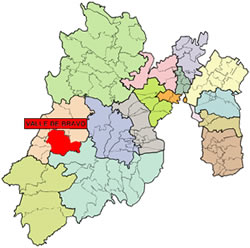
\includegraphics[width=0.35\textwidth]{valle.jpg}
\end{wrapfigure}
\section{Introducción}
Primeramente y como introducción, en esta actividad nos enfocamos en el uso de la biblioteca Pandas en el contexto de análisis de datos. El análisis se realizo sobre los datos meteorológicos de Valle de Bravo, un municipio del estado de México, los cuales fueron proporcionados por el Servicio Meteorológico Nacional. \\
Se eligió este municipio en particular por contar con un amplio registro de datos, lo cual arrojara mejores resultados al hacer un análisis estadístico. \\
En la actividad se aplicaron distintas funciones de la biblioteca de Pandas, así como otras bibliotecas auxiliares para la realización de graficas. \\
En base al análisis, se busco responder distintas preguntas, sobre los niveles de precipitación y temperaturas registradas en las últimas décadas: \\
1. ¿Cómo le podrás determinar cuáles son los meses más lluviosos? \\
2. ¿Cuáles son los meses más fríos y cuáles son los más cálidos? \\
3. ¿Cuáles han sido años muy húmedos? \\
4. ¿Cuáles han sido años muy secos? \\
5. ¿Cuáles años han tenido inviernos fríos? \\
6. ¿Cuáles años han tenido veranos más cálidos? \\
7. ¿Cómo ha venido siendo la temperatura mensual promedio en los últimos 20 años? \\
8. ¿Qué ha pasado con la precipitación en los últimos 20 años de datos? 


\section{Desarrollo de la actividad}
\subsection{Metodología}
Una vez obtenido el archivo de texto con los datos de Valle de Bravo, se creo un nuevo archivo en Jupyter Notebook, al cual se importan las siguientes librerías:

\begin{center}
\textcolor{ForestGreen} {import} plotly.plotly \textcolor{ForestGreen}{as} py\\
\textcolor{ForestGreen} {import} plotly.tools \textcolor{ForestGreen} {as} tls\\
\textcolor{ForestGreen} {import} matplotlib.pyplot \textcolor{ForestGreen} {as} plt; plt.rcdefaults()\\
\textcolor{ForestGreen} {import} pandas \textcolor{ForestGreen} {as} pd\\
\textcolor{ForestGreen} {import} numby \textcolor{ForestGreen} {as} np\\


\end{center}Estas nos ayudaran con los cálculos matemáticos, el análisis estadístico y la realización de graficas, para poder leer los datos, evitando los valores nulos, a estos se les asigno una variable.

\begin{center}
\begin{verbatim} sentinels = {'PRECIP': ['Nulo'],'EVAP':['Nulo'],'TMAX':['Nulo'],'TMIN':['Nulo']} \end{verbatim}
\end{center}
Después se leyó el archivo mediante el comando “pd.read\_csv”, y posteriormente se creo un Data Frame mediante el comando “pd.DataFrame()”.
Como el archivo cuenta con una columna de fechas, a esta se le dio formato de fecha mediante:

\begin{center}
\begin{verbatim} df['FECHAN'] = pd.to\_datetime(df.apply(lambda x: x['FECHA'], 1), dayfirst=True)
    
    df = df.drop(['FECHA'], 1)
    \end{verbatim}
\end{center}
Para dar solución a las preguntas planteadas se emplearon diversas funciones sobre el Data Frame.

\begin{table}[]
\centering
\caption{Funciones de Data Frame empleadas.}
\begin{tabular}{|c|c|}
\hline
Función         & Acción              \\ \hline
df.head()       & Encabezado          \\ \hline
df.tail()       & Final               \\ \hline
df.dtypes()     & Tipos de variables  \\ \hline
df.mean()       & Promedio            \\ \hline
df.std()        & Desviación Estándar \\ \hline
df.median()     & Mediana             \\ \hline
df.max()        & Máximo              \\ \hline
df.min()        & Mínimo              \\ \hline
df.describe()   & Resumen estadístico \\ \hline
df.drop()       & Eliminar            \\ \hline
df.apply()      & Aplicar función     \\ \hline
df.idxmax()     & Máximo (índice)     \\ \hline
df.idxmin()     & Mínimo (índice)     \\ \hline
df.iloc()       & Mostrar índice      \\ \hline
df.loc()        & Accesar             \\ \hline
df.isin()       & Selección           \\ \hline
df.unique()     & Valores diferentes  \\ \hline
df.snsmallest() & N menores           \\ \hline
df.nlargest()   & N mayores           \\ \hline
\end{tabular}
\end{table}
También se utilizó polyplot para realiza gráficas, y así lograr una mejor interpretación de los datos.


\newpage
\subsection{Resultados}
\noindent\textbf {1. ¿Cómo le podrás determinar cuáles son los meses más lluviosos?} \\
\begin{center}
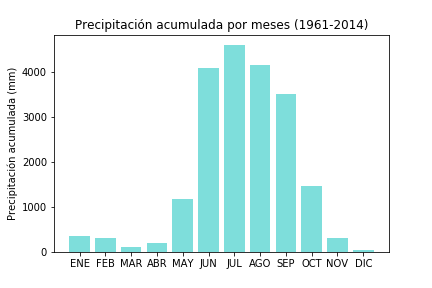
\includegraphics[scale=0.65]{Precipit_mensual.png}
\end{center}
Para determinar esto se calculó la suma de precipitaciones totales para cada mes de todos los años. Se realizó una gráfica de barras con los resultados. Aquí se puede apreciar que los meses más lluviosos han sido Junio, Julio y Agosto.\\\\

\noindent\textbf {2. ¿Cuáles son los meses más fríos y cuáles son los más cálidos?} \\
\begin{center}
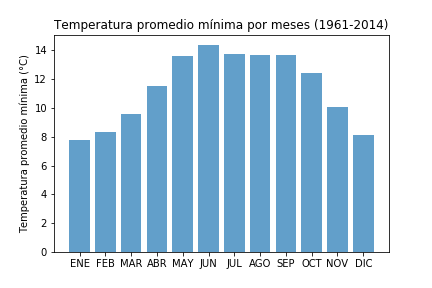
\includegraphics[height=5cm]{Temperaturaprommin_mensual.png}
\hspace*{\fill}
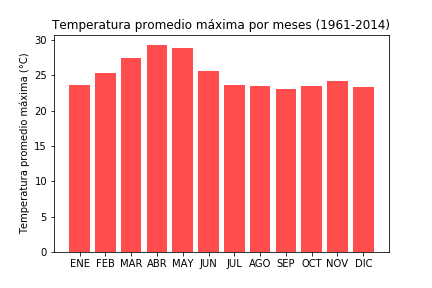
\includegraphics[height=5cm]{Temperaturapromax_mensual.png}
\end{center}
Para saber cuáles fueron los meses más fríos y cálidos se calculó el promedio de las temperaturas máximas y mínimas de manera mensual. 
En base a ellas podemos afirmar que los meses con temperaturas más bajas son Diciembre, Enero y Febrero. 
En cambio, los meses con temperaturas más altas son Marzo, Abril y Mayo.
\\

\noindent\textbf {3. ¿Cuáles han sido años muy húmedos?, ¿Cuáles han sido años muy secos?, ¿Qué ha pasado con la precipitación en los últimos 20 años de datos?} \\
\begin{center}
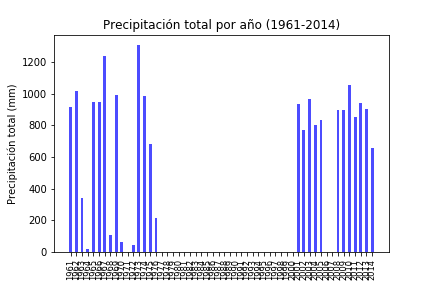
\includegraphics[scale=0.65]{Precip_anual.png}
\end{center} Para responder a esto se realizó un nuevo Data Frame con dos columnas. La primera columna contiene un arreglo de los años, y la segunda contiene la suma de precipitaciones para cada año. Al observar la gráfica correspondiente notamos que 1964, 1971, 1972, 1977-2000 y 2006-2007 fueron años muy secos, mientras que 1962, 1967, 1973 y 2010 han sido los años más lluviosos. Observando la información, vemos que las precipitaciones han ido aumentando en los últimos 20 años, pero es notable que en las décadas anteriores llovía mas que en las actúales. \\


\noindent\textbf {4. ¿Cuáles años han tenido inviernos fríos?}
\begin{center}
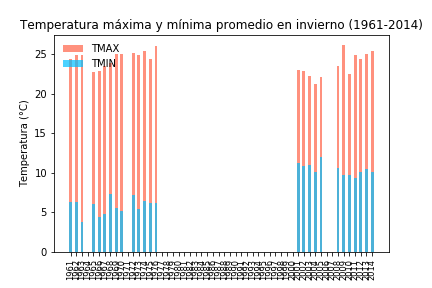
\includegraphics[scale=0.65]{Temperaturasprom_invierno.png}
\end{center} 
En la gráfica se observa que 1963, 1966 y 1967 fueron los años que han tenido los inviernos con temperaturas mas bajas de lo que regularmente es. \\



\noindent\textbf {5. ¿Cuáles años han tenido veranos más cálidos?} \\
\begin{center}
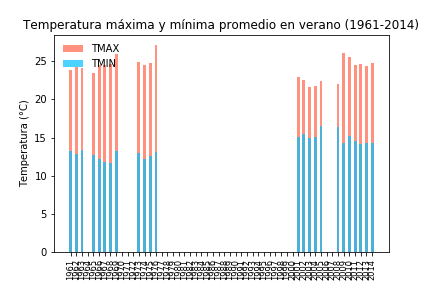
\includegraphics[scale=0.65]{Temperaturasprom_verano.png}
\end{center} Se seleccionaron los datos de los meses de verano de cada año, y se calculó el promedio de temperaturas máximas y mínimas.
De aquí podemos observar que los años con temperaturas más altas han sido 1969, 1976 y 2009. \\


\noindent\textbf {6. ¿Cómo ha venido siendo la temperatura mensual promedio en los últimos 20 años?} \\
\begin{center}
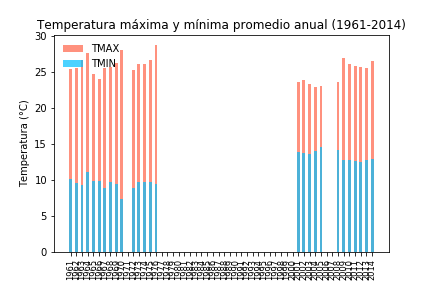
\includegraphics[scale=0.65]{Temperaturasprom_anual.png}
\end{center} Debido a la extensión de los datos, se realizó un promedio de las temperaturas máximas y mínimas de manera anual. Podemos observar que las temperaturas mínimas han sido cada vez mas altas y las temperaturas maximas tambien han aumentado.


\section{Conclusiones}
Podemos concluir que a partir de las gráficas observamos que desde 1961 hasta 2014 han aumentado la temperatura y las precipitaciones en el municipio de Valle de Bravo. También observamos que, la época de lluvias se da en los meses de Junio, Julio y Agosto. Estos resultados son congruentes con lo esperado, ya que los cambios de temperatura y precipitación observados pueden atribuirse al calentamiento del planeta debido al cambio climático en las ultimas décadas.

\section{Referencias}
\begin{itemize}
\item El Servicio Meteorológico Nacional, Información Estadística Climatológica,\\ Recuperado de: https://smn.cna.gob.mx/es/climatologia/informacion-climatologica/informacion-estadistica-climatologica
\item Pandas Cookbook. Recuperado de:\\ http://pandas.pydata.org/pandas-docs/stable/user\_guide/cookbook.html\#cookbook
\item How do you convert data frame column to int in python. Recuperado de:\\
https://stackoverflow.com/questions/51898361/how-do-you-convert-data-frame-column-to-int-in-python
\end{itemize}

\end{document}